\section{Kontinuerlig simulering}
\thispagestyle{fancy}

Undervegs i programmeringa har vi utført kontinuerlege testar og simuleringar av blokkene vi har utvikla, noko
som har våre ein viktig del av arbeidsmetodane vi har brukt i oppgåva. 

Kontinuerleg simulering er små testar som blir utførte medan ein programmerar.
Det er ikkje ein isolert testfase med klare start- og stoppunkt, men heller små kontinuerlege testar og verifiseringar som gir oss ein indikasjon
på om arbeidet følgjer spesifikasjon.

I denne oppgåva nytta vi kontinuerleg simulering i programmeringsfasen av \gls{IEC} blokkene.
Desse blokkene hadde mange funksjonar som ikkje nødvendigvis var avhengige av kvarandre,
som gjorde det mogleg å gjennomføra små, enkle testar på dei ulike områda utan at heile blokka var ferdigstilt.\newline
Som eit døme, skal \gls{RX} resette ein utgang \gls{Y}. Dette blir implementert og deretter testa ved hjelp av simulering.
Kva som til slutt skal sette utgangen \gls{Y} høg er ikkje relevant i dette tilfellet. Vi har likevel implementert 
og testa at ein reset vil fungere.


\begin{figure}[htbp]
    \centering
    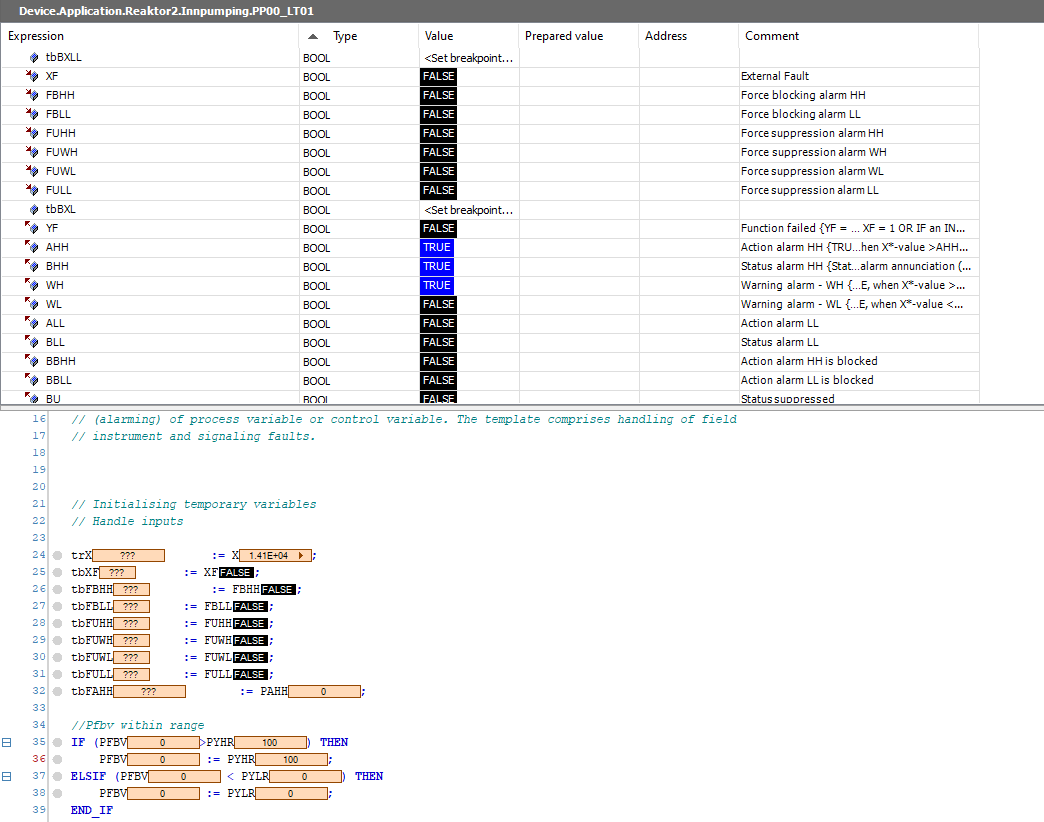
\includegraphics[width=0.8\textwidth]{Bilder/kontinuerligSimulering.png}
    \caption{Kontinuerleg testing ved manipulasjon av verdiar}\label{fig:KontinuerlegSimulering}
\end{figure}


\newpage
